\hspace{0.5 cm}
Pentru a putea înțelege mai bine cum funcționează rețeaua neuronală din cadrul \textbf{Benchmark-ul cGAN al competiției VNN-Comp 2023} este necesar să înțelegem cum funcționează în general o rețea de tipul GAN, iar apoi una de tip cGAN.
\begin{itemize}
    \item \textbf{GAN}(Generative Adversarial Networks) este un model neuronal mai special \cite{GAN} a cărui concept poate fi reprezentat ca un joc între două rețele neuronale distincte adversare.

    \item \textbf{cGAN}(Conditional GAN) \cite{CGAN} ghidează procesul de creare a datelor prin încorporarea unor etichete specificice în GAN ca cele două rețele neuronale adversare să se poată orienta după acestea.
\newline
\end{itemize}

O reprezentare grafică a rețelei neuronale din cadrul Benchmark-ul cGAN al competiției VNN-Comp 2023 ar arăta în felul următor:


\begin{figure}[ht]
\centering
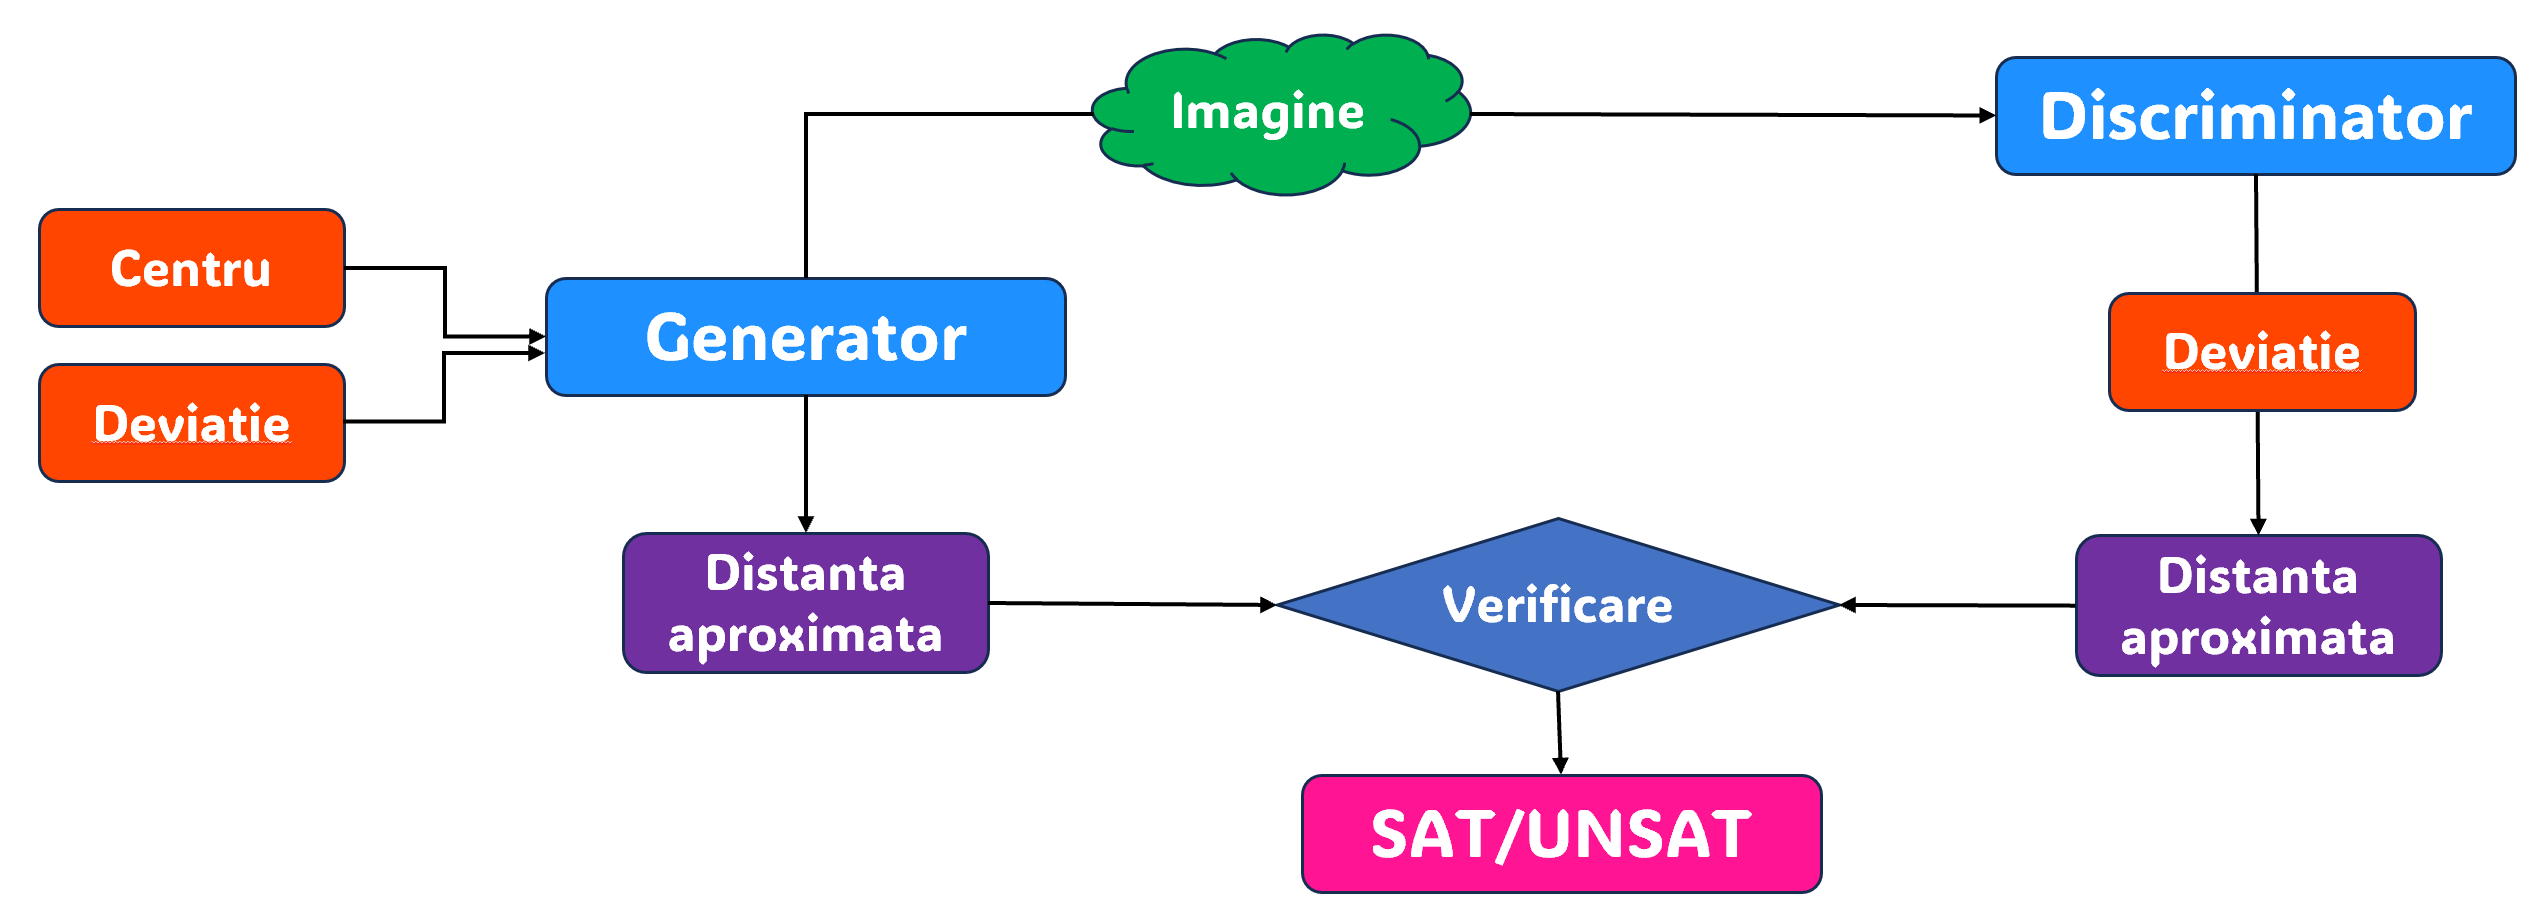
\includegraphics[width=12cm]{imagini/introducere/Ale_1.png}
\caption{Reprezentare grafică a rețelei neuronale din cadrul Benchmark-ul cGAN al competiției VNN-Comp 2023}
\label{reprezentare_grafica_cGAN}
\end{figure}

Conform graficului, Fig.\ref{reprezentare_grafica_cGAN}, în cazul acestei rețele neuronale cele două rețele distincte adversare se împart în:

\begin{itemize}
  \item \textit{Generatorul} - pe baza pe datele de intrare(adică etichetele), are rolul de a genera o valoare reprezentată de o distanță și o imagine cu un obstacol aflat la o acea distanță
  
  \item \textit{Discriminatorul} - pe baza imaginii returnate de generator, are rolul de a aproxima distața până la obstacol
\end{itemize}
\newpage

Iar datele de intrare sunt:

\begin{itemize}
  \item \textit{Etichetele} -  sunt reprezentate de condiția de distanță și un vector de zgomot, care practic funcțiomnează ca un fel de centru și o deviație
\end{itemize}

Evaluarea performanței acestei rețele se concentrează pe capacitatea ei de a genera conținut condiționat. În particular, verificarea se bazează pe  alinierea distanței prezise de discriminator cu condiția distanței de intrare oferită de generator.

De exemplu, pentru o înțelegere mai clara, am construit următorul exemplu:


\begin{figure}[ht]
\centering
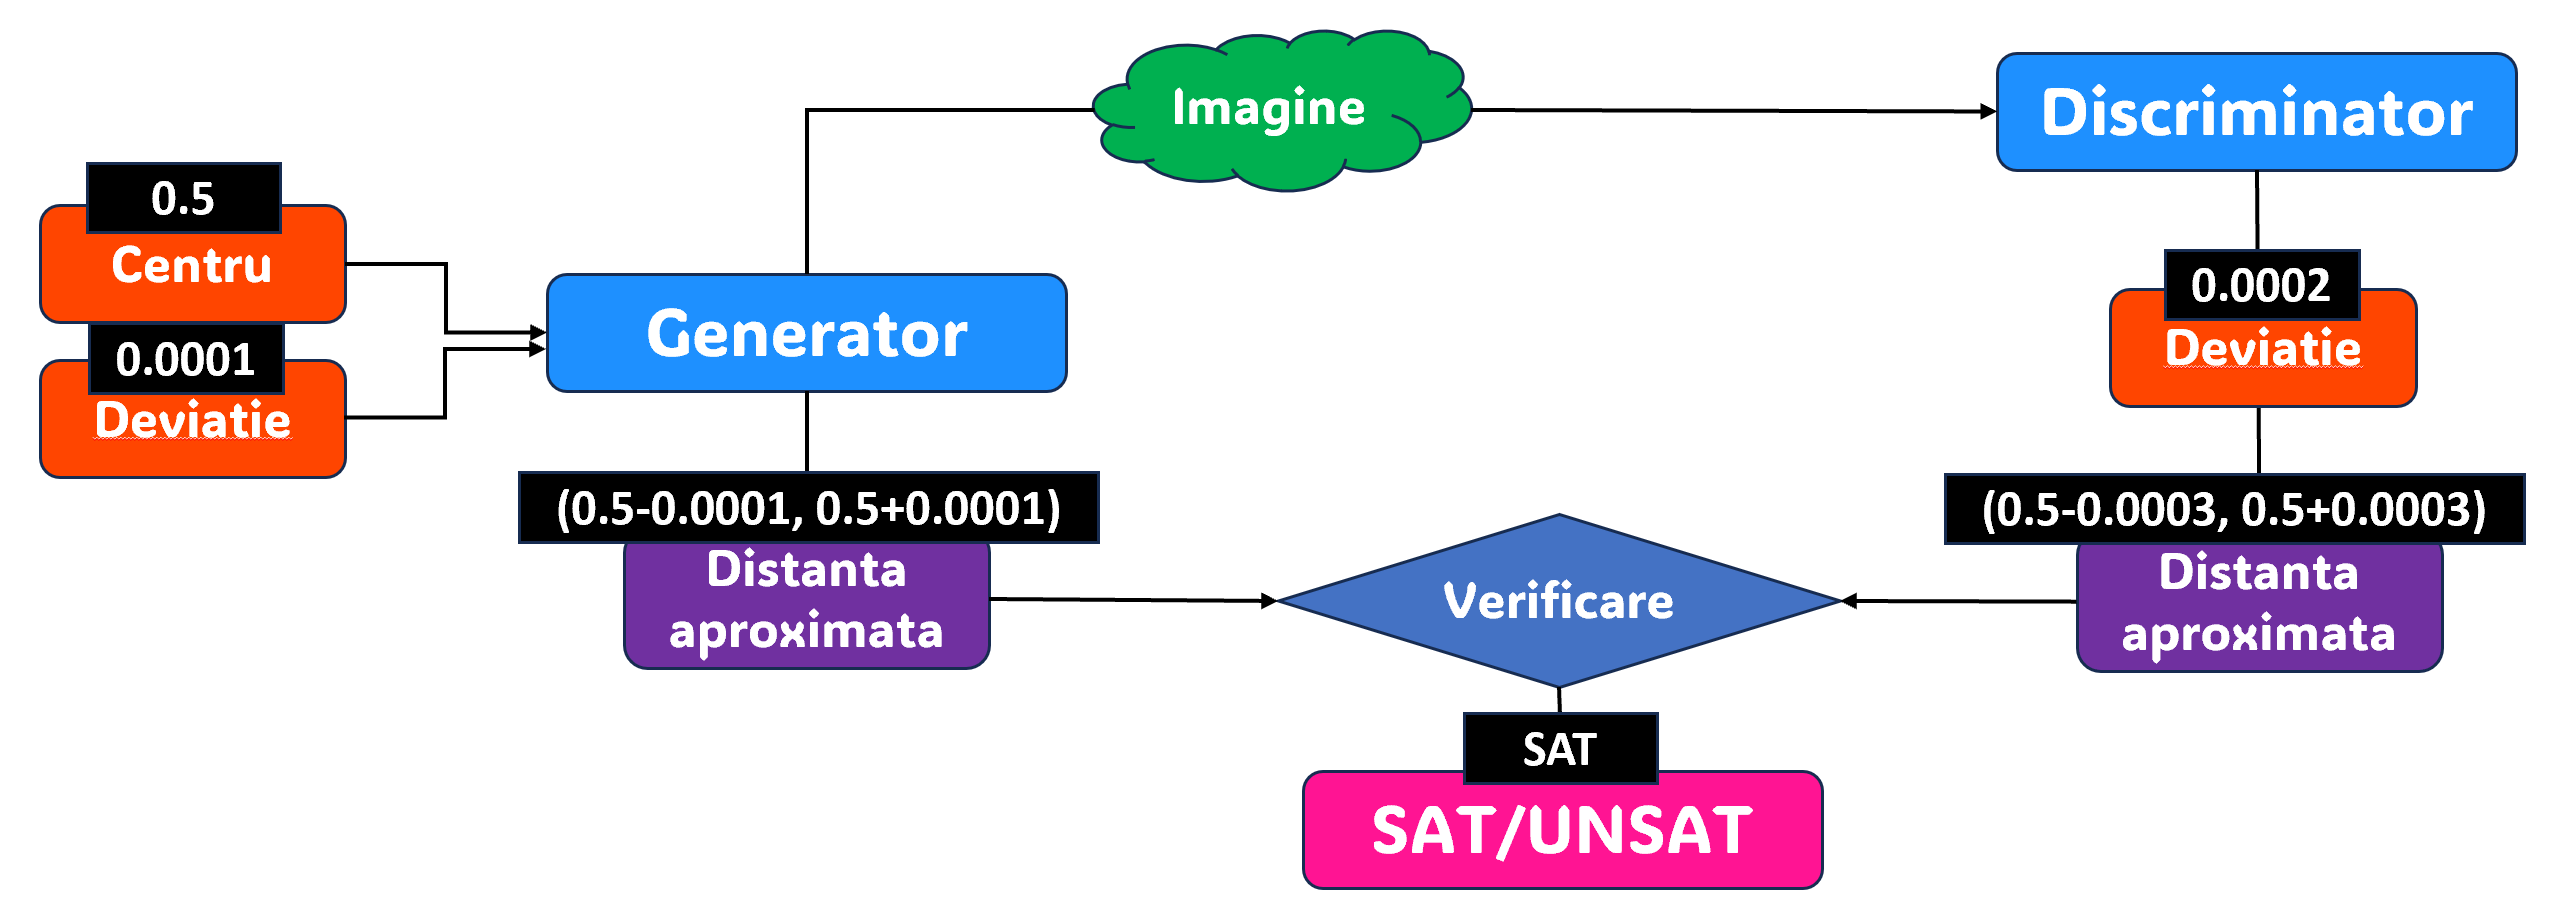
\includegraphics[width=12.5cm]{imagini/introducere/Ale_2.png}
\caption{Reprezentare grafică a rețelei neuronale din cadrul Benchmark-ul cGAN al competiției VNN-Comp 2023 - exemplu de date de intrare}
\label{reprezentare_grafica_cGAN_exemplu}
\end{figure}

În exemplul de mai sus, Fig.\ref{reprezentare_grafica_cGAN_exemplu}, să presupunem că pentru datele de intrare avem un centru de 0,5 și o deviație de 0,0001. Prin urmare, intervalul distanței la care se poate afla obstacolul este de (0,5-0,0001, 0,5+0,0001). 

Obiectivul nostru este să ne asigurăm că distanța prezisă de discriminator se potrivește cu acest interval. Mai exact, distanța prezisă de discriminator trebuie să se situeze în intervalul de intrare adăugând din nou o deviație, de data asta să zicem 0,0002, adică putem obține o distanță aproximativă în intervalul (0,5-0,0003, 0,5+0,0003).

Dacă obținem din partea discriminatorului o distanță din acel interval, acest lucru indică faptul că \textbf{imaginile generate respectă condiția de distanță de intrare}.

Rezultatul acestei verificări returnează un rezultat \textbf{satisfiabil} dacă se indică o \textbf{aproximare corectă a distanței de către discriminator}, în caz contrar se obține un rezultat \textbf{nesatisfiabil}.
\newpage